\section{Design}

\subsection{Runtime Cluster}

\begin{figure}[!t]
\begin{subfigure}[t]{0.30\linewidth}
   \centering
   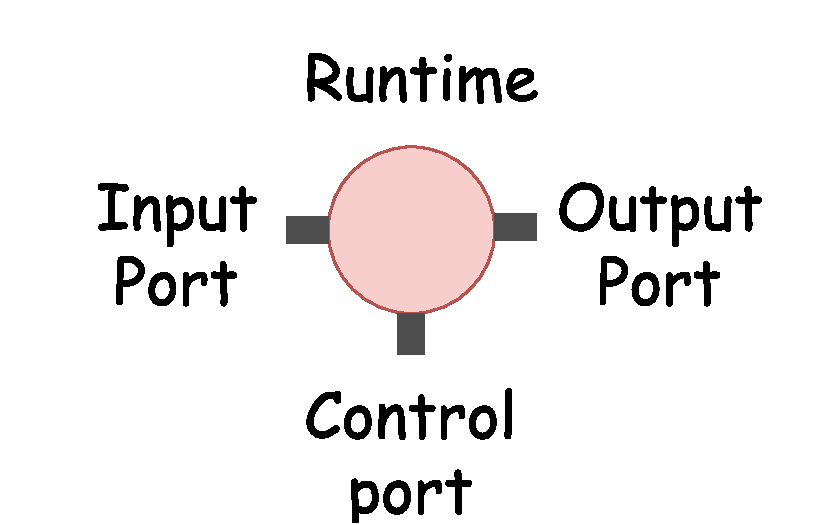
\includegraphics[width=\columnwidth]{figure/nfactor-runtime-with-port.pdf}
   \caption{A runtime with three ports.}\label{fig:rep-scale}
  \end{subfigure}\hfill
  \begin{subfigure}[t]{0.69\linewidth}
 \centering
   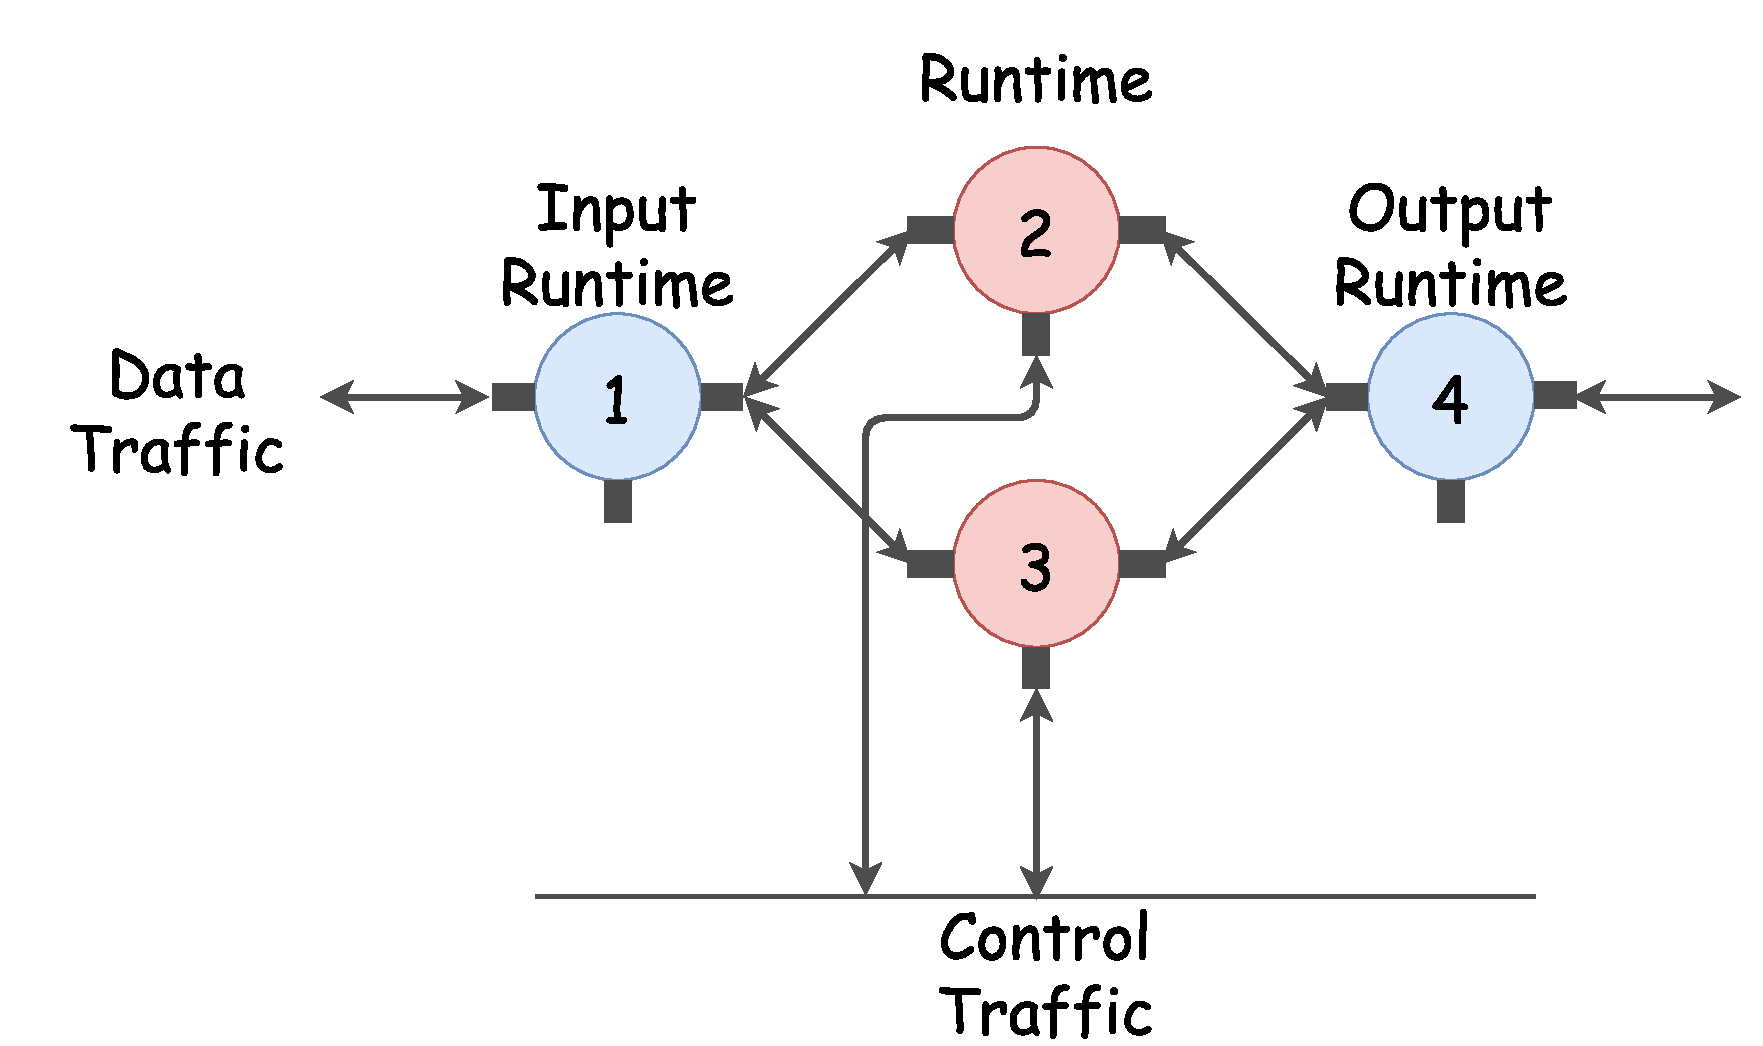
\includegraphics[width=\columnwidth]{figure/nfactor-runtime-connection.pdf}
   \caption{A runtime connected with an input runtime and an output runtime.}\label{fig:rep-recovery} \end{subfigure}\hfill
   \begin{subfigure}[t]{0.99\linewidth}
  \centering
    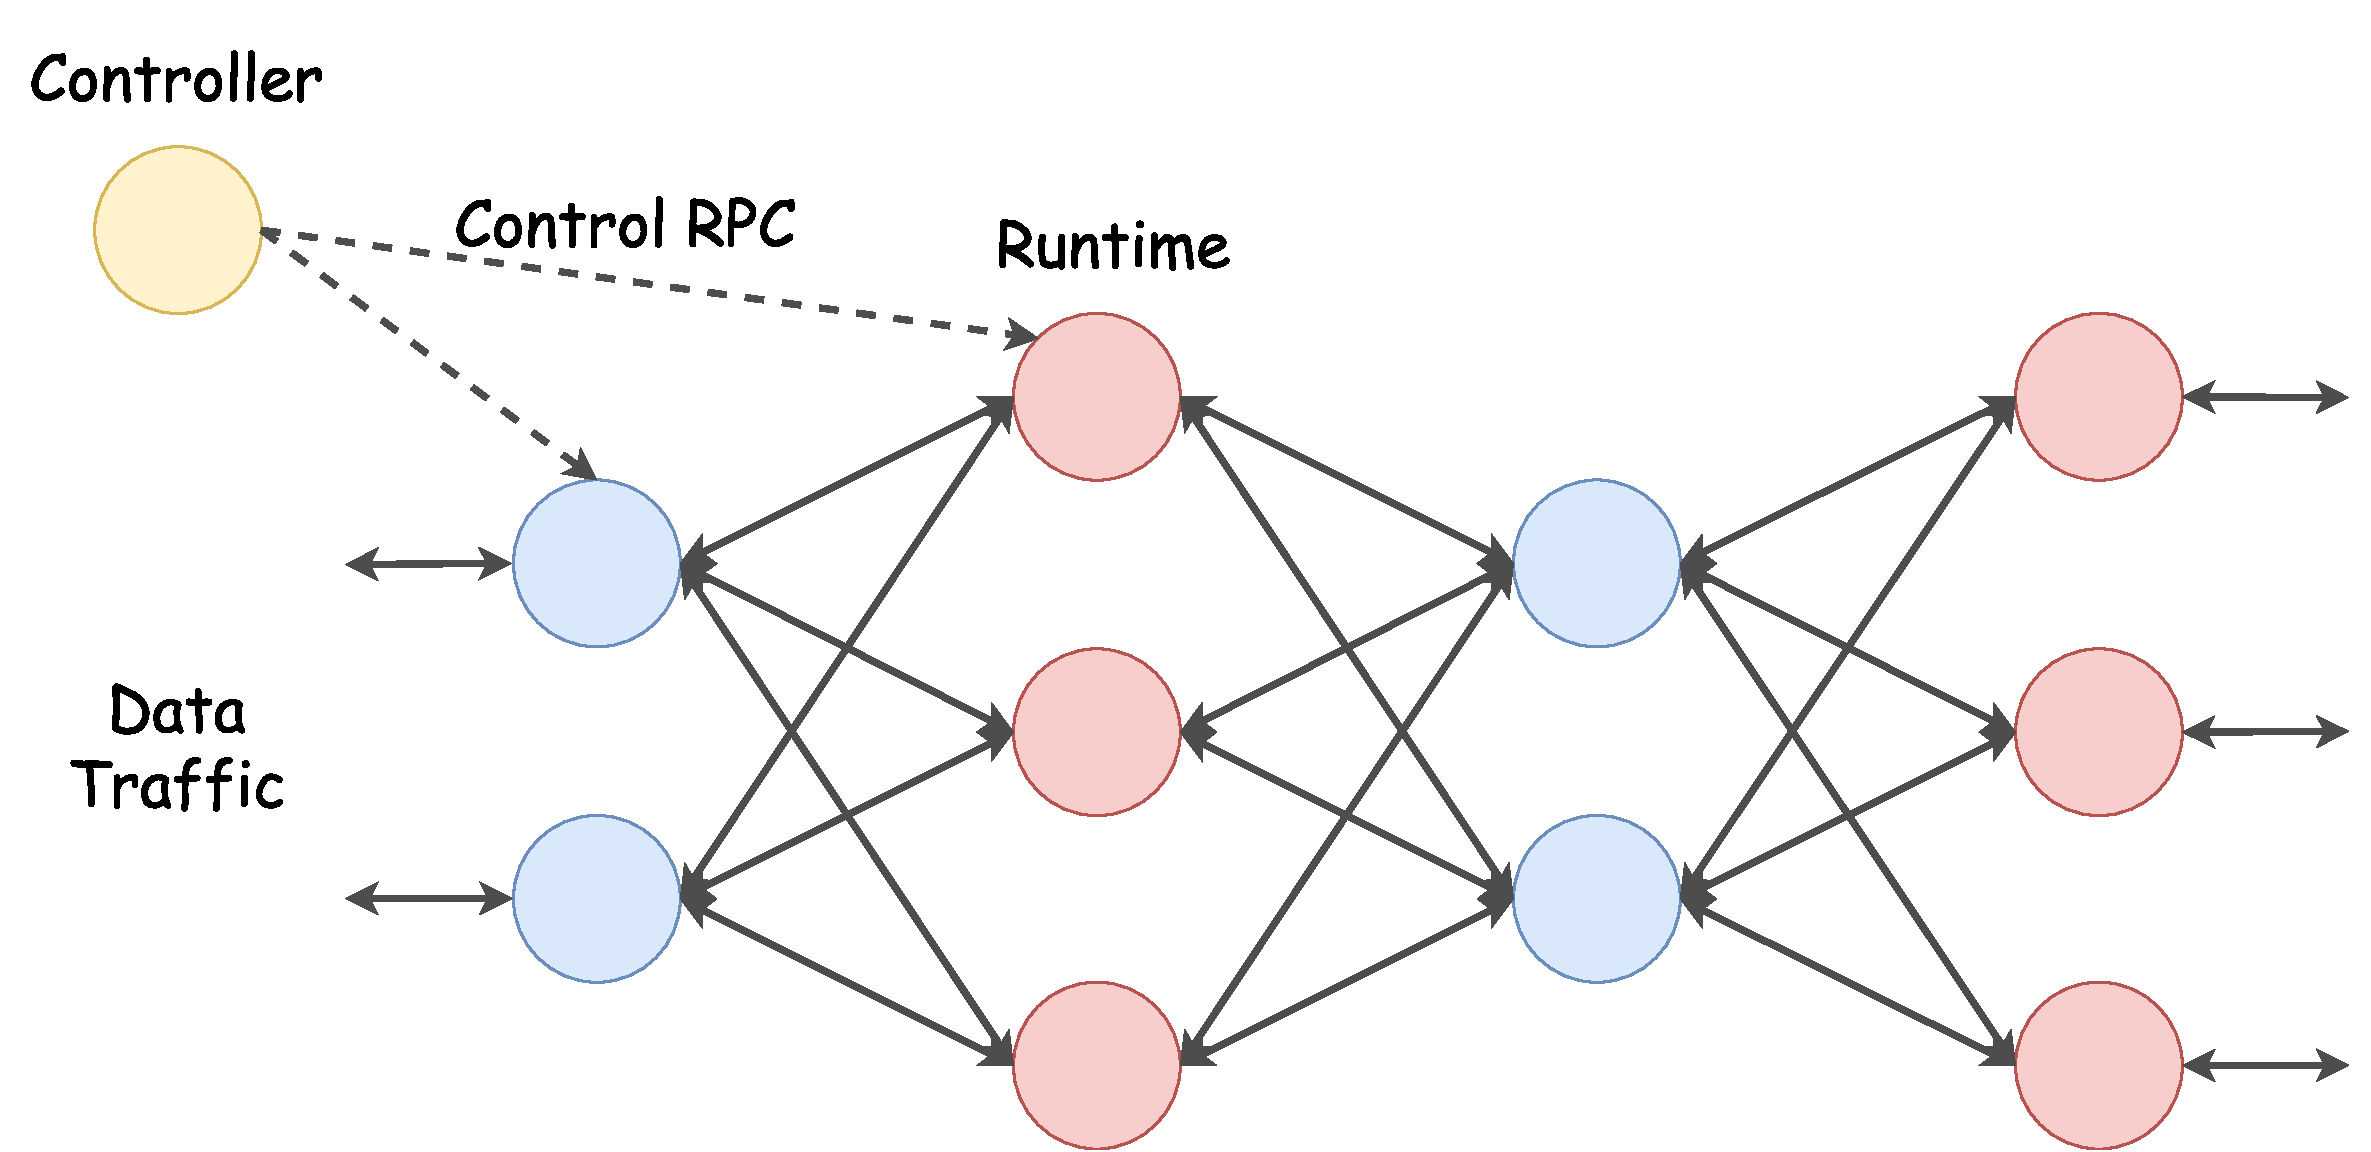
\includegraphics[width=\columnwidth]{figure/nfactor-cluster.pdf}
    \caption{A NFActor runtime cluster controlled by a controller.}\label{fig:rep-recovery} \end{subfigure}
 \caption{The flow migration performance of \nfactor}
\label{fig:rep-perf}
\end{figure}
